%styl klasy z Polskimi Normami oprac. Marcin Wolinski
\documentclass[a4paper,titleauthor]{mwart} 

\usepackage{polski}
\usepackage[utf8]{inputenc}
\usepackage{graphicx} %pakiet do wstawiania grafiki
\usepackage[hyphens]{url} %pakiet do wstawiania linkow
%\usepackage[hidelinks,breaklinks]{hyperref}
\usepackage{authblk}%pakiet do tworzenia afiliacji
\usepackage{tabularx}%pakiet do tabel
\usepackage[a4paper, left=2cm, right=2cm, top=3cm, bottom=3cm]{geometry}
\usepackage{listings}
\usepackage{placeins}%pakiet do kontroli umieszczania obiektow
\usepackage{hyperref}%pakiet do m.in. kolorowania linkow
\usepackage{amsmath}%pakiet do matematyki np. równania na parę linijek
\usepackage{float}%opcja [H] dla figur, zostają tam gdzie wstawiło je się w tekście
\hypersetup{pdfborder=0 0 0}

\usepackage[sorting=none]{biblatex}
% \addbibresource{bibl}
% \bibliography{bibl}

\usepackage{changepage}



% \documentclass[a4paper,11pt]{article}

% \usepackage[cp1250]{inputenc}

\usepackage[tablegrid,owncaptions]{vhistory}
\renewcommand{\vhhistoryname}{Historia zmian}
\renewcommand{\vhversionname}{Wersja}
\renewcommand{\vhdatename}   {Data}
\renewcommand{\vhauthorname} {Autor}
\renewcommand{\vhchangename} {Opis zmian}

\renewcommand\figurename{Rys.}%skrocony podpis
\renewcommand\lstlistingname{Wydruk}
\renewcommand\refname{Bibliografia}



%------------------------------------------------------------------------
% Dane do strony tytułowej

\title{{\Huge  Projekt KRYS}\\ - \\{\Large Szyfr blokowy  SM4 }\\ }



\author{Gabriela Maciejewska \and Sławomir Nikiel \and Aleksandra Krawczyk \vspace{25em}}




\affil{Politechnika Warszawska,\\ Wydział Elektroniki i Technik Informacyjnych} % Wyrzuciłem instytut, bo nie mój ;]
\date{27.11.2021}

%------------------------------------------------------------------------
% Początek dokumentu
\begin{document}
	
%Automatycznie generowany tytuł dokumentu
\maketitle

%------------------------------------------------------------------------

%------------------------------------------------------------------------
% Automatycznie generowany spis treści
\newpage
\tableofcontents







%------------------------------------------------------------------------
%pliki z rodzialami
\newpage
\section{Wstęp}

Zasada chaosu i zasada dyfuzji to dwie podstawowe zasady projektowania szyfrów blokowych. Dobrze zaprojektowany algorytm szyfru blokowego powinien opierać się na kryptograficznie uzasadnionej strukturze transformacji podstawowej.
Kryptograficzne właściwości transformacji podstawowej decydują o efektywności wynikowej transformacji szyfrującej.
Algorytm SM4 jest zbudowany na permutacji ortomorficznej. Jego transformacja rundy jest permutacją ortomorficzną, a jego właściwości kryptograficzne można wydedukować z właściwości tej permutacji.
\section{Rys historyczny}

Algorytm „SMS4” został wymyślony przez Shu-Wang Lu. Po raz pierwszy został opublikowany w 2003 r. jako część 	"Information technology -- Telecommunications and information exchange between systems -- Local and metropolitan area networks -- Specific requirements -- Part 11: Wireless LAN Medium Access Control (MAC) and Physical Layer (PHY) Specifications", a następnie opublikowany niezależnie w 2006 r. przez SCA(State Cryptography Administration of China) (wówczas OSCCA - Office of State Commercial Cryptography Administration) jako SMS4 - Cryptographic Algorithm For Wireless LAN Products. Został opublikowany jako branżowy standard kryptograficzny i przemianowany na „SM4” w 2012 r. przez SCA, a ostatecznie sformalizowany w 2016 roku jako Chiński Standard Narodowy - "Information security technology -- SM4 block cipher algorithm".\\

SM4 został pierwotnie stworzony do użytku w ochronie sieci bezprzewodowych i jest zgodny z chińskim National Standard for Wireless LAN WAPI (Wired Authentication and Privacy Infrastructure), czyli alternatywą dla mechanizmów bezpieczeństwa określonych w IEEE 802.11i.
Został przedłożony Międzynarodowej Organizacji Normalizacyjnej ISO przez Chińskie Stowarzyszenie Normalizacyjne SAC. \\

Zarówno WAPI, jak i IEEE 802.11i zostały zaproponowane jako poprawki bezpieczeństwa do normy ISO/IEC 8802-11.
Oba schematy wykorzystują dwa różne szyfry blokowe do szyfrowania danych:
- WAPI wykorzystuje szyfr blokowy SMS4, podczas gdy IEEE 802.11i używa szyfru blokowego AES. \\

W marcu 2006 roku IEEE 802.11i został zatwierdzony jako ISO/IEC 8802-11 WLAN, natomiast WAPI został częściowo odrzucony, ze względu na nieujawniomy szyfr SMS4. Jednakże, ponieważ WAPI jest nadal oficjalnie wymagany dla chińskiego standardu krajowego,
jest nadal używany w chińskiej branży WLAN i wielu międzynarodowych
korporacjach, takich jak SONY, które wspierają WAPI w odpowiednich produktach. \\



Najnowszy standard SM4 został zaproponowany przez SCA (wówczas OSCCA), znormalizowany przez TC 260 Administracji Normalizacyjnej Chińskiej Republiki Ludowej (SAC) i został opracowany przez następujące osoby w Centrum Badań Danych i Bezpieczeństwa Komunikacji (Centrum DAS) Chińskiej Akademii Nauk, Chińskie Centrum Testowania Kryptografii Komercyjnej oraz Pekińska Akademia Informatyki i Technologii (BAIST):

\begin{itemize}
    \item Shu-Wang Lu
    \item Dai-Wai Li
    \item Kai-Yong Deng
    \item Chao Zhang
    \item Peng Luo
    \item Zhong Zhang 
    \item Fang Dong
    \item Ying-Ying Mao
    \item Zhen-Hua Liu
\end{itemize}


SM4 został również ostatecznie znormalizowany w ISO/IEC 8802-11 przez Międzynarodową Organizację Normalizacyjną w 2017 r.















\section{Opis szyfru\cite{4}}
% opis szyfru, jaka jest jego struktura, jakie prymitywy wykorzystuje, jakie parametry

SM4 to chiński standard szyfrowania blokowego, wprowadzony do ochrony sieci bezprzewodowych i wydany w styczniu 2006 roku. Wejście, wyjście i klucz SM4 mają 128 bitów.
Algorytm ma 32 rundy, z których każda modyfikuje jedno z czterech 32-bitowych słów. Szyfrowanie i
deszyfrowanie ma tę samą strukturę, z wyjątkiem tego, że klucz do deszyfrowania to
odwrotność klucza do szyfrowania.

\subsection{Definicje}

Następujące definicje są kluczowe do opisania struktury szyfru SM4.

\subsubsection{Słowo i bajt}

Zdefiniujmy $Z^{e}_{2}$ jako zbiór e-bitowych wektorów. Słowo wykorzystywane w algorytmie szyfrowania SM4 jest elementem $Z^{32}_{2}$, natomiast bajt elementem $Z^{8}_{2}$.

\subsubsection{S box}

S box, czyli blok podmiany (ang. substitution), przyjmuje 8 bitów na wejściu i zwraca 8 bitów na wyjściu. 

\subsubsection{Podstawowe operacje}

Podstawowymi operacjami bitowymi używanymi w omawianym algorytmie są:
\begin{enumerate}
    \item $\oplus$ --- bitowy XOR dwóch wektorów z $Z^{32}_{2}$
    \item $<<< \textit{i}$ --- obrót bitowy w lewo o \textit{i} bitów
\end{enumerate}

\subsubsection{Wejście, wyjście i klucz}

Tekst jawny to 128-bitowy blok składający się z czterech 32-bitowych słów $X = (X_0, X_1, X_2, X_3)$. Szyfrogram to analogiczny do tekstu jawnego 128-bitowy blok składający się z czterech 32-bitowych słów $Y = (Y_0, Y_1, Y_2, Y_3)$.

Klucz podawany do szyfru również zachowuje tę samą konwencję $MK = (MK_0, MK_1, MK_2, MK_3)$. Używany jest do generowania zestawu kluczy rund $(rk_0, rk_1, \ldots, rk_{31})$, gdzie $rk_i \in Z^{32}_2$.

\subsection{Funkcja rundy F}

Niech blok $(X_0, X_1, X_2, X_3) \in (Z^{32}_2)^4$ będzie 128-bitowym wejściem oraz $rk \in Z^{32}_2$ kluczem rundy, wówczas funkcja $F: (Z^{32}_2)^5 \rightarrow Z^{32}_2$:
\begin{equation*}
F(X_0, X_1, X_2, X_3, rk) = X_0 \oplus T(X_1 \oplus X_2 \oplus X_3 \oplus rk)
\end{equation*}

\begin{figure}[h!]
  \centering
  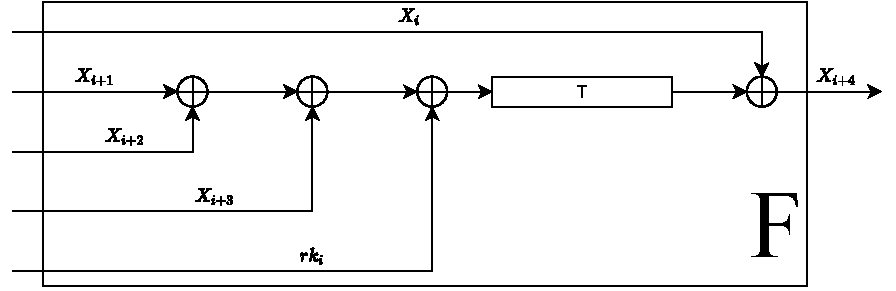
\includegraphics{diagramy/F.pdf}
  \caption{Blok F}
  \label{fig:F}
\end{figure}

\subsubsection{Mieszane podstawienie T}

$T: Z^{32}_2 \rightarrow Z^{32}_2$ jest odwracalną funkcją podstawienia. Składa się z nieliniowego podstawienia $\tau$ oraz liniowego  $L$.
\begin{equation*}
    T(\ldots) = L(\tau(\ldots))
\end{equation*}

\paragraph{Nieliniowe podstawienie $\tau$}\mbox{}

Niech $A$ będzie 32-bitowym słowem wejściowym, czyli $A = (a_0, a_1, a_2, a_3) \in (Z^8_2)^4$. Wówczas $\tau: (Z^8_2)^4 \rightarrow (Z^8_2)^4$ definiujemy następująco:

\begin{equation*}
    \tau(A) = (Sbox(a_0), Sbox(a_1), Sbox(a_2), Sbox(a_3))
\end{equation*}

\paragraph{Liniowe podstawienie $L$}\mbox{}

Niech B, będzie wynikiem otrzymanym z funkcji $\tau$. Wówczas funkcja $L: Z^{32}_2 \rightarrow Z^{32}_2$ definiowana jest następująco:

\begin{equation*}
    L(B) = B \oplus (B <<< 2)  \oplus (B <<< 10)  \oplus (B <<< 18)  \oplus (B <<< 24) 
\end{equation*}

\subsubsection{S box}

Działanie S boxa opisuje tabela \ref{table:sbox}. Wartości przedstawione są w systemie heksadecymalnym.

\begin{table}[h!]
\centering
\caption{S box}
\label{table:sbox}
\begin{tabular}{ | c | cccccccccccccccc | } 
\hline
 & 0 & 1 & 2 & 3 & 4 & 5 & 6 & 7 & 8 & 9 & a & b & c & d & e & f \\
\hline
0 & d6 & 90 & e9 & fe & cc & e1 & 3d & b7 & 16 & b6 & 14 & c2 & 28 & fb & 2c & 05 \\
1 & 2b & 67 & 9a & 76 & 2a & be & 04 & c3 & aa & 44 & 13 & 26 & 49 & 86 & 06 & 99 \\
2 & 9c & 42 & 50 & f4 & 91 & ef & 98 & 7a & 33 & 54 & 0b & 43 & ed & cf & ac & 62 \\
3 & e4 & b3 & 1c & a9 & c9 & 08 & e8 & 95 & 80 & df & 94 & fa & 75 & 8f & 3f & a6 \\
4 & 47 & 07 & a7 & fc & f3 & 73 & 17 & ba & 83 & 59 & 3c & 19 & e6 & 85 & 4f & a8 \\
5 & 68 & 6b & 81 & b2 & 71 & 64 & da & 8b & f8 & eb & 0f & 4b & 70 & 56 & 9d & 35 \\
6 & 1e & 24 & 0e & 5e & 63 & 58 & d1 & a2 & 25 & 22 & 7c & 3b & 01 & 21 & 78 & 87 \\
7 & d4 & 00 & 46 & 57 & 9f & d3 & 27 & 52 & 4c & 36 & 02 & e7 & a0 & c4 & c8 & 9e \\
8 & ea & bf & 8a & d2 & 40 & c7 & 38 & b5 & a3 & f7 & f2 & ce & f9 & 61 & 15 & a1 \\
9 & e0 & ae & 5d & a4 & 9b & 34 & 1a & 55 & ad & 93 & 32 & 30 & f5 & 8c & b1 & e3 \\
a & 1d & f6 & e2 & 2e & 82 & 66 & ca & 60 & c0 & 29 & 23 & ab & 0d & 53 & 4e & 6f \\
b & d5 & db & 37 & 45 & de & fd & 8e & 2f & 03 & ff & 6a & 72 & 6d & 6c & 5b & 51 \\
c & 8d & 1b & af & 92 & bb & dd & bc & 7f & 11 & d9 & 5c & 41 & 1f & 10 & 5a & d8 \\
d & 0a & c1 & 31 & 88 & a5 & cd & 7b & bd & 2d & 74 & d0 & 12 & b8 & e5 & b4 & b0 \\
e & 89 & 69 & 97 & 4a & 0c & 96 & 77 & 7e & 65 & b9 & f1 & 09 & c5 & 6e & c6 & 84 \\
f & 18 & f0 & 7d & ec & 3a & dc & 4d & 20 & 79 & ee & 5f & 3e & d7 & cb & 39 & 48 \\
\hline
\end{tabular}
\end{table}

Przykładowo dla wejścia '3f' odczytujemy 3-ci rząd i f-ą kolumnę: $Sbox('3f') = a6$. Sbox bazuje na operacji odwracania nad ciałem $GF(2^8)$ --- Ciało Galois.

\subsection{Kodowanie i dekodowanie}

Niech $R$ będzie odwrotnym podstawieniem:

\begin{equation*}
    R(A_0, A_1, A_2, A_3) = (A_3, A_2, A_1, A_0), A_i \in Z^{32}_2, i = 0, 1, 2, 3
\end{equation*}

Weźmy tekst jawny $(X_0, X_1, X_2, X_3) \in (Z^{32}_2)^4$, oznaczmy jego szyfrogram jako $(Y_0, Y_1, Y_2, Y_3) \in (Z^{32}_2)^4$. Załóżmy, że klucze poszczególnych rund zostały wygenerowane z klucza 128-bitowego i są definiowane jak następuje: $rk_i \in Z^{32}_2, i = 0,1, \ldots, 31$. Szczegóły generowania kluczy rund opisane są w sekcji \ref{section:roundKeys}.

Kodowanie przebiega w następujący sposób:

\begin{equation*}
    X_{i+4} = F(X_i, X_{i+1}, X_{i+2}, X_{i+3}, rk_i) = X_i \oplus T(X_{i+1} \oplus X_{i+2} \oplus X_{i+3} \oplus rk_i), i = 0,1,\ldots,31
\end{equation*}
        
\begin{equation*}
    (Y_0, Y_1, Y_2, Y_3) = R(X_{32}, X_{33}, X_{34}, X_{35})
\end{equation*}

Dekodowanie odbywa się za pomocą tego samego algorytmu, jedyną różnicą jest odwrotna kolejność kluczy rund. Klucze rund kodowania $(rk_0, rk_1, \ldots, rk_{31})$, klucze rund dekodowania $(rk_{31}, rk_{30}, \ldots, rk_0)$

\begin{figure}[H]
  \centering
  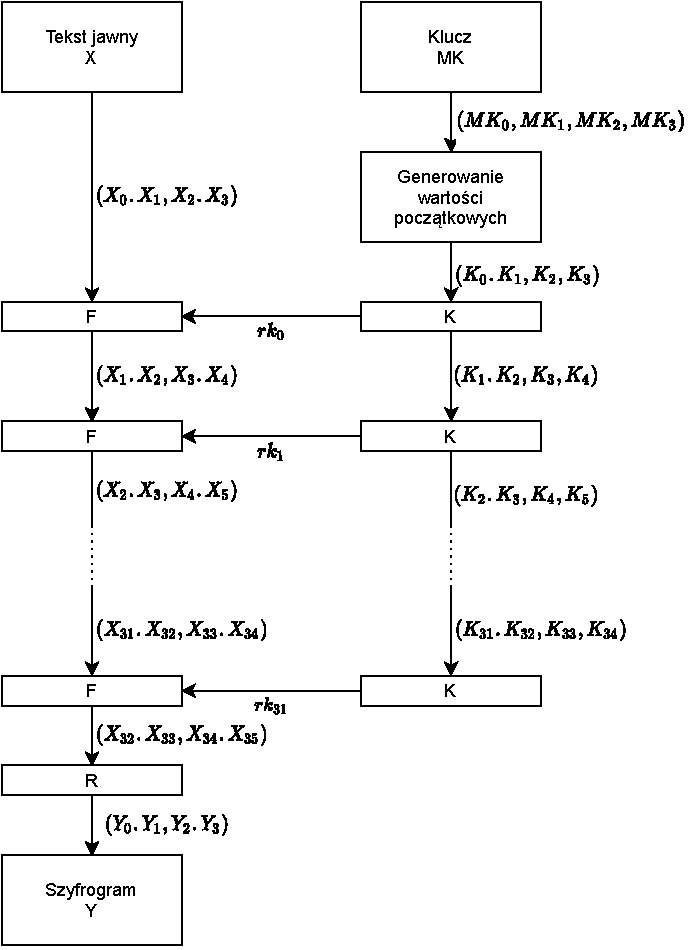
\includegraphics{diagramy/SM4.pdf}
  \caption{Schemat algorytmu szyfrowania SM4}
  \label{fig:SM4}
\end{figure}

Bloki F i K opisane są kolejno na Rysunku \ref{fig:F} i Rysunku \ref{fig:K}.

\subsection{Generowanie kluczy rund} \label{section:roundKeys}

Klucze rund generowane są z klucza 128-bitowego. Niech $MK = (MK_0, MK_1, MK_2, MK_3), MK_i \in Z^{32}_2, i = 0, 1, 2, 3$ będzie głównym kluczem 128-bitowym. Wówczas klucze rund $rk_i \in Z^{32}_2, i = 0, 1, \ldots, 31$ otrzymywane są w następujący sposób.
\begin{equation*}
    (K_0, K_1, K_2, K_3) = (MK_0 \oplus FK_0, MK_1 \oplus FK_1, MK_2 \oplus FK_2, MK_3 \oplus FK_3)
\end{equation*}

 Wówczas dla $i = 0, 1, \ldots, 31$:
\begin{equation*}
    rk_i = K_{i+1} = K_i \oplus T'(K_{i+1} \oplus K_{i+2} \oplus K_{i+3} \oplus CK_i)
\end{equation*}

\begin{figure}[H]
  \centering
  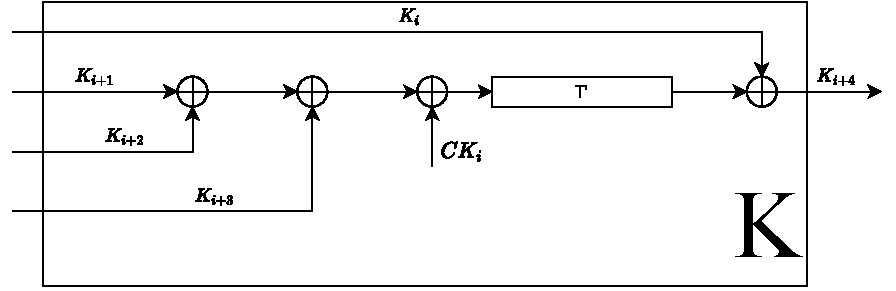
\includegraphics{diagramy/K.pdf}
  \caption{Blok K}
  \label{fig:K}
\end{figure}

\paragraph{Mieszane podstawienie T'}\mbox{}

Podstawienie T' jest defniowane tak samo jak podstawienie T z tą różnicą, że zamianst funkcji L używana jest następująca funkcja L':

\begin{equation*}
    L'(B) = B \oplus (B <<< 13) \oplus (B <<< 23)
\end{equation*}

\paragraph{Parametr FK}\mbox{}

Przytaczane parametry FK zdefiniowane są w notacji heksadecymalnej:

\begin{equation*}
    FK_0 = (a3b1bac6), FK_1 =  (56aa3350), FK_2 = (677d9197), FK_3 = (b27022dc)
\end{equation*}

\paragraph{Parametr CK}\mbox{}

Niech $ck_{i,j}$ będzie j-tym bajtem $CK_i = (ck_{i,0}, ck_{i,1}, ck_{i,2}, ck_{i,3}) \in (Z^8_2)^4$, gdzie $ck_{i,j} = (4i + j) \times 7 \pmod{256}$. Z tego wynika, że parametry CK są stałymi i nie ma potrzeby każdorazowego obliczania ich.









\section{Analiza bezpieczeństwa}

Od czasu pierwszej publikacji, SM4 został poddany wielu kryptoanalizom wykonanym przez międzynarodowych badaczy. Obecnie, nie są jednak znane żadne praktyczne ataki na pełny szyfr SM4. Jedyne pojawiające się obawy związane z kanałami bocznymi \cite{1}, gdy algorytm używany jest w implementacji sprzętowej. \\

SM4 został przeanalizowany pod względem następujących typów ataków:
\begin{itemize}
    \item liniowe - kryptoanaliza liniowa jest jedną z najważniejszych technik analizy kryptograficznej z kluczem symetrycznym. Kryptoanaliza liniowa skupia się na liniowości przybliżenia między tekstem jawnym, tekstem zaszyfrowanym i kluczem. Jeśli szyfr zachowuje się inaczej niż losowa permutacja można zbudować wyróżnik lub nawet atak odzyskiwania klucza poprzez dodanie kilku rund. Podklucze dołączonych rund są odgadywane, a szyfrogramy są odszyfrowywane i/lub jawne teksty są szyfrowane przy użyciu tych podkluczy do obliczenia stanu pośredniego na końcach wyróżnika.
    \item różnicowe - kryptoanaliza różnicowa, jest jednym z najpotężniejszych ataków na wybrany tekst jawny (lub wybrany tekst szyfrujący) w kryptografii symetryczno-kluczowej (tzn. w szyfrach blokowych, szyfrach strumieniowych, funkcjach haszujących i algorytmach MAC). Po wprowadzeniu tego ataku, został on skutecznie zastosowany do wielu znanych szyfrów, a także zaproponowano różne warianty tego ataku (atak na obciętą różnicę, atak na kwadrat, atak na różniczkę, atak na niemożliwą różnicę, atak na bumerang).
    \item liniowe wielowymiarowe - Biryukov et al. \cite{2} zaproponował podejście, które może wykorzystywać wiele aproksymacji liniowych z różnymi bitami klucza. Jednakże, metody te zakładają, że aproksymacje liniowe są statystycznie niezależne.
    \item niemożliwe różnicowe - w porównaniu z normalnymi atakami różnicowymi, niemożliwy atak różnicowy jest bardziej efektywny w przypadku niektórych szyfrów blokowych, takich jak np. AES. Zastosowanie w SMS4 jest również kolejnym skutecznym sposobem atakowania tuż po atakach różnicowych.
    \item algebraiczne - Kryptoanaliza algebraiczna polega na znalezieniu i rozwiązaniu układu równań wielomianowych wielowartościowych w skończonym polu.
    \item liniowe o zerowej korelacji,
    \item integralne,
    \item macierzowe. \\
\end{itemize} 


Porównanie najsilniejszych ataków na algorytm SM4 znajduje się w tabeli \ref{table:attacks}. Obecnie nie są powszechnie znane żadne skuteczne ataki powyżej 24 rundy.

\begin{table}[h!]
\centering
\caption{Najsilniejsze ataki na SM4}
\label{table:attacks}
\begin{tabular}{ | c | cccc | } 
\hline
 Metoda & Rundy & Złożoność czasu & złożoność danych & złożoność pamięci \\
\hline
$Linear$ & 24 & 2^{122.6} & 2^{122.6} & 2^{85} \\
$Multi-dimensional$ $Linear$ & 23 & 2^{122.7} & 2^{122.6} & 2^{120.6}\\
$Differential$ & 23 & 2^{126.7} & 2^{117} & 2^{120.7}\\
$Matrix$ & 18 & 2^{110.77} & 2^{127} & 2^{130}\\
$Impossible$ $Differential$ & 17 & 2^{132} & 2^{117} & --\\
$Zero-correlation$ $Linear$ & 14 & 2^{120.7} & 2^{123.5} & 2^{73}\\
$Integral$ & 14 & 2^{96.5} & 2^{32} & --\\
$Brute force$ & 11 & 2^{128} & 2^{128} & --\\
\hline
\end{tabular}
\end{table}
Na podstawie danych zamieszczonych w tabeli możemy stwierdzić, że atak brutalny nie jest skutecznym sposobem ataku w przypadku algorytmu SM4. Umożliwia on dotarcie tylko do 11 rundy przy bardzo wysokich wartościach złożoności czasowej i danych.

Kwestie bezpieczeństwa są w Chinach niezwykle istotne. Produkty i usługi wykorzystujące kryptografię są regulowane przez SCA \cite{3} - muszą one być wyraźnie zatwierdzone lub certyfikowane przez SCA zanim zostaną dopuszczone do sprzedaży lub użytkowania w Chinach. Algorytm SM4 jest uważany tam za alternatywę dla AES-128.

\subsection{ Atak liniowy \cite{6}}
 Aby przeprowadzić atak liniowy (atak na odzyskiwanie klucza) na 24-rundowe SM4 dodajemy dwie rundy odpowiednio na dole i na górze 20-rundowej aproksymacji liniowej w tabeli \ref{table:linear}. Technika sum częściowych \cite{5} jest używana w procedurach częściowego szyfrowania i deszyfrowania. Cały proces przedstawiony jest na rysunku \ref{fig:KeyRecoveryAttack}.\\
 Zgodnie z aproksymacją liniową oznaczamy, że $\Gamma^{0}_{2} = \Gamma^{3}_{2} = \Gamma^{0}_{22} = \Gamma^{3}_{22} = 0x8808A288, \Gamma^{1}_{2} =0x8808C228, \Gamma^{2}_{2} = \Gamma^{1}_{22} = 0x88080828, \Gamma^{2}_{22} = 0x88086828, \Lambda_{1}= \Lambda_{22} = 0x00008200,  \Lambda_{1,2} =  \Lambda_{22,2}= 0x82.$ \\
 Z liniowego przybliżenia wynika, że
 \begin{equation*}
   \Gamma^{0}_{2} \cdot X^{0}_{2} \oplus \Gamma^{1}_{2} \cdot X^{1}_{2} \oplus \Gamma^{2}_{2} \cdot X^{2}_{2} \oplus \Gamma^{3}_{2} \cdot X^{3}_{2} \oplus \Gamma^{0}_{22} \cdot X^{0}_{22} \oplus \Gamma^{1}_{22} \cdot X^{1}_{22} \oplus \Gamma^{2}_{22} \cdot X^{2}_{22} \oplus \Gamma^{3}_{22} \cdot X^{3}_{22} = K
\end{equation*}

Rozważmy częściowe szyfrowanie i deszyfrowanie, wtedy lewą stronę  powyższego równania można zapisać w następujący sposób:
\begin{equation*}
   \Gamma^{0}_{2} \cdot P_{2} \oplus \Gamma^{1}_{2} \cdot P_{3} \oplus \Gamma^{2}_{2} \cdot (P_{0} \oplus XX_{0}) \oplus \Gamma^{0}_{2} \cdot (P_{1} \oplus XX_{1}) \oplus \Gamma^{0}_{2} \cdot (C_{2} \oplus XX_{22}) \oplus \Gamma^{2}_{2} \cdot (C_{3} \oplus XX_{23}) \oplus \Gamma^{2}_{22} \cdot C_{0} \oplus \Gamma^{0}_{2} \cdot C_{1} =  
\end{equation*}
\begin{equation*}
   \Gamma^{0}_{2} \cdot P_{2} \oplus \Gamma^{1}_{2} \cdot P_{3} \oplus \Gamma^{2}_{2} \cdot P_{0} \oplus \Gamma^{0}_{2} \cdot P_{1} \oplus \Gamma^{0}_{2} \cdot C_{2} \oplus \Gamma^{2}_{2} \cdot C_{3} \oplus \Gamma^{2}_{22} \cdot C_{0} \oplus \Gamma^{0}_{2} \cdot C_{1} \oplus \Gamma^{2}_{2} \cdot XX_{0} \oplus \Gamma^{0}_{2} \cdot XX_{1} \oplus \Gamma^{0}_{2} \cdot XX_{22} \oplus \Gamma^{2}_{2}\cdot XX_{23},
\end{equation*}

gdzie $XX_r$ jest stanem po transformacji T, a $XS_r$  jest stanem po warstwie $S$ w r-tej rundzie.

\begin{equation*}
   \Theta = \Gamma^{0}_{2} \cdot P_{2} \oplus \Gamma^{1}_{2} \cdot P_{3} \oplus \Gamma^{2}_{2} \cdot P_{0} \oplus \Gamma^{0}_{2} \cdot P_{1} \oplus \Gamma^{0}_{2} \cdot C_{2} \oplus \Gamma^{2}_{2} \cdot C_{3} \oplus \Gamma^{2}_{22} \cdot C_{0} \oplus \Gamma^{0}_{2} \cdot C_{1}.
\end{equation*}
Atak odzyskiwania klucza przebiega w następujący sposób:\\
\begin{enumerate}
    \item Zbierz N par tekstu jawnego i odpowiadającego mu szyfrogramu.\\
    \item Inicjalizuj $2^{82}$ liczników $V_0[0]$, ..., $V_0[2^{81}-1]$ do zera.\\
    \item Dla każdej pary tekstu jawnego i odpowiadającego mu szyfrogramu oblicz:
    \begin{equation*}
   w = \Theta || (P_{1} \oplus P_{2} \oplus P_{3})  || (C_{3} \oplus C_{0} \oplus C_{1}) || C_{0} \oplus C_{1} \oplus C_{2} || P_{1} \oplus P_{2} \oplus P_{3}.
   \end{equation*} 
   Następnie zwiększ licznik $V_0[w]$ o jeden.\\
    \item Odgadnij 32-bitowe $k_{23}$.Zaalokuj $2^{49}$ liczników $V_1[0]$, ..., $V_1[2^{49}-1]$ na zero.\\
    \item Dla każdego $0\leq w \leq 2^{81}-1 $ oblicz $\Theta \Leftarrow \Theta \oplus \Gamma^{2}_{2} \cdot T(C_{0} \oplus C_{1} \oplus C_{2} \oplus k_{23}), XX_{23}$ oraz $x=\Theta || (P_{0} \oplus P_{2} \oplus P_{3}) || (C_{3} \oplus C_{0} \oplus C_{1}) \oplus XX_{23} || P_{1} \oplus P_{2} \oplus P_{3}. V_1[x]+=V_0[w]$.\\
    \item Odgadnij 8-bitowe $k_{22}$. Zainicjuj $2^{41}$ liczników $V_2[0]$, ..., $V_2[2^{41}-1]$ na zero.\\
    \item Dla każdego $0\leq x \leq 2^{49}-1 $ oblicz $\Theta \Leftarrow \Theta \oplus \Lambda_{1,2} \cdot S((C_{3} \oplus C_{0} \oplus C_{1})\oplus XX_{23} \oplus k_{22})$ oraz $y=\Theta || (P_{0} \oplus P_{2} \oplus P_{3}) || P_{1} \oplus P_{2} \oplus P_{3}). V_2[y]+=V_1[x]$.\\
    \item Odgadnij 32-bitowe $k_0$. Zainicjuj $2^{9}$ liczników $V_3[0]$, ..., $V_3[2^{9}-1]$ na zero.\\
    \item Dla każdego $0\leq y \leq 2^{41}-1 $ oblicz $\Theta \Leftarrow \Theta \oplus \Gamma^{2}_{2} \cdot T(P_{1} \oplus P_{2} \oplus P_{3} \oplus k_{0}), XX_{0}]$ oraz $z=\Theta || (P_{0} \oplus P_{2} \oplus P_{3}) \oplus XX_{0}. V_3[z]+=V_2[y]$.\\
    \item Odgadnij 8-bitowe $k_1$. Zainicjuj $2^{80}$ liczników $V_1[0]$, ..., $V_1[2^{80}-1]$ na zero.\\
    \item Dla każdego $0\leq z \leq 2^{9}-1 $ oblicz $\Theta \Leftarrow \Theta \oplus \Lambda_{1,2} \cdot S((P_{1} \oplus P_{2} \oplus P_{3})\oplus XX_{0} \oplus k_{1})$. Jeśli $\Theta =0$ zwiększ $V_{key}[k_0 || k_1 || k_{22} || k_{23}]$ o $V_3[z]$, w przeciwnym przypadku zmniejsz go o $V_3[z]$.\\
    \item Ustaw przewagę $\alpha$ na 47, co oznacza, że zachowane są $2^{33}$ największe wartości bezwzględne w $V_{key}$. Dla każdej zachowanej wartości podklucza, zgadujemy pozostałe 88 bitów z $k_1[0-15, 24-31] || k_2 || k_3$ (klucz główny można uzyskać z harmonogramu kluczy) i przetestować klucz przez ścieżkę szyfrowania.\\
\end{enumerate}

\begin{table}[h!]
\centering
\caption{Aproksymacja liniowa dla 20-rundowego SM4}
\label{table:linear}
\begin{tabular}{ | c | cccccccc | } 
\hline
 Rundy & i & \Gamma^{0}_{i} & \Lambda_{i} & \Gamma_{i} &  tendencyjność & \Gamma^{1}_{i} & \Gamma^{2}_{i} & \Gamma^{3}_{i}\\
\hline
$1$ & 0 & 8808A228 & 00008200 & 00006000 & 2^{-4} & 8808C228 & 88080828 & 8808A228\\
$2$ & 1 & 8808A228 & 00008200 & 0000CA00 & 2^{-4} & 88086828 & 8808C228 & 8808A228\\
$3$ & 2 & 8808A228 & 00008200 & 0000AA00 & 2^{-4} & 88080828 & 88086828 & 8808A228\\
$4$ & 3 & 8808A228 & 00008200 & 00006000 & 2^{-4} & 8808C228 & 88080828 & 8808A228\\
$5$ & 4 & 8808A228 & 00008200 & 0000CA00 & 2^{-4} & 88086828 & 8808C228 & 8808A228\\
$6$ & 5 & 8808A228 & 00008200 & 0000AA00 & 2^{-4} & 88080828 & 88086828 & 8808A228\\
$7$ & 6 & 8808A228 & 00008200 & 00006000 & 2^{-4} & 8808C228 & 88080828 & 8808A228\\
$8$ & 7 & 8808A228 & 00008200 & 0000CA00 & 2^{-4} & 88086828 & 8808C228 & 8808A228\\
$9$ & 8 & 8808A228 & 00008200 & 0000AA00 & 2^{-4} & 88080828 & 88086828 & 8808A228\\
$10$ & 9 & 8808A228 & 00008200 & 00006000 & 2^{-4} & 8808C228 & 88080828 & 8808A228\\
$11$ & 10 & 8808A228 & 00008200 & 0000CA00 & 2^{-4} & 88086828 & 8808C228 & 8808A228\\
$12$ & 11 & 8808A228 & 00008200 & 0000AA00 & 2^{-4} & 88080828 & 88086828 & 8808A228\\
$13$ & 12 & 8808A228 & 00008200 & 00006000 & 2^{-4} & 8808C228 & 88080828 & 8808A228\\
$14$ & 13 & 8808A228 & 00008200 & 0000CA00 & 2^{-4} & 88086828 & 8808C228 & 8808A228\\
$15$ & 14 & 8808A228 & 00008200 & 0000AA00 & 2^{-4} & 88080828 & 88086828 & 8808A228\\
$16$ & 15 & 8808A228 & 00008200 & 00006000 & 2^{-4} & 8808C228 & 88080828 & 8808A228\\
$17$ & 16 & 8808A228 & 00008200 & 0000CA00 & 2^{-4} & 88086828 & 8808C228 & 8808A228\\
$18$ & 17 & 8808A228 & 00008200 & 0000AA00 & 2^{-4} & 88080828 & 88086828 & 8808A228\\
$19$ & 18 & 8808A228 & 00008200 & 00006000 & 2^{-4} & 8808C228 & 88080828 & 8808A228\\
$20$ & 19 & 8808A228 & 00008200 & 0000CA00 & 2^{-4} & 88086828 & 8808C228 & 8808A228\\
$21$ & 20 & 8808A228 & 00008200 & * & * & 88080828 & 88086828 & 8808A228\\
\hline
\end{tabular}
\end{table}

Złożoność czasowa kroku (3) wynosi około $2^{126.6}$ operacji, co jest równoważne $2^{126.6}/24 = 2^{122.0}$ 24-rundom
szyfrowania. Kroki (5) i (9) wymagają $2^{113}$ jednokrotnych
deszyfracji lub szyfrowania. Kroki (7) i (11) wymagają $2^{89}$
jednokrotnych odszyfrowań lub zaszyfrowań. Złożoność
kroku (12) wynosi $2^{121}$ 24-rund szyfrowań. Zatem całkowita złożoność czasowa wynosi około $2^{126.6}$ szyfrowań.
Złożoność pamięciowa kroku (2) wynosi około $2^{81}\times8 = 2^{84}$ bajtów, a licznik $Vkey$ wymaga $2^{80}\times 16 = 2^{84}$  bajtów, więc
całkowita złożoność pamięciowa wynosi około $2^{84}+2^{84}=2^{85}$  bajtów.\\
Przy złożoności danych $2^{126.6}$, prawdopodobieństwo sukcesu tego ataku wynosi 76.1\%.

 \begin{figure}[h!]
  \centering
  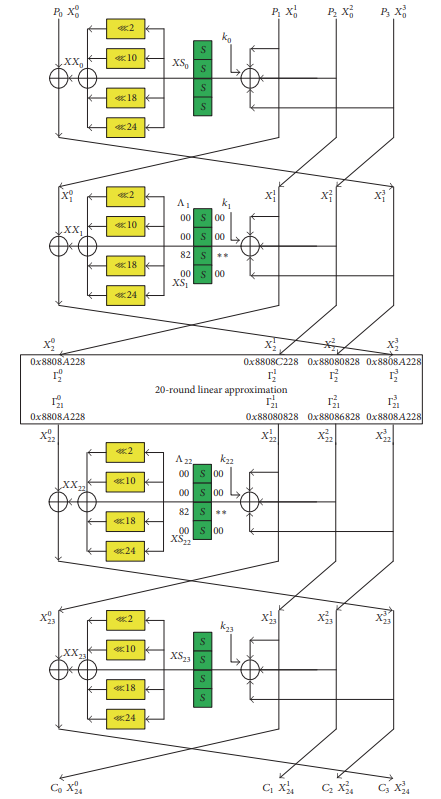
\includegraphics{diagramy/KeyRecoveryAttack.png}
  \caption{Atak odzyskiwania klucza na 24-rundowy SM4}
  \label{fig:KeyRecoveryAttack}
\end{figure}

\section{Analiza efektywności}

Efektywność algorytmu jest jedną z jego podstawowych cech. Możemy wyróżnić złożoność czasową i pamięciową algorytmu i na tej podstawie wybrać, który algorytm jest dla nas bardziej korzystny ze względu na czas, albo na złożoność pamięciową.\\

\subsection{ Złożoność czasowa}
Złożoność czasowa – to ilość czasu potrzebnego do wykonania zadania, wyrażona jako funkcja ilości danych, aby ją określić należy rozważyć złożoność poszczególnych operacji oraz ilość ich powtórzeń. Wynik powinien być sprawdzony dla każdej możliwej kombinacji wejściowej. Funkcja złożoności czasowej: t: {0, 1}* → N nazywamy złożonością czasową algorytmu A, jeżeli dla każdego x na wejściu algorytm zatrzymuje się po x krokach dokładnie w t(x). Jeśli funkcja otrzymuje skończoną liczbę danych wejściowych, to jej złożoność czasowa wynosi O(1), zależy więc od rozmiaru danych.\\

Złożoność czasowa funkcji SM4:
\begin{itemize}
    \item funkcja rundy F -  funkcja otrzymuje pięć 32-bitowych wektorów i zwraca jeden 32 bitowy wektor, podczas tej funkcji wykonywane są 4 operacje XOR dwóch 32 bitowych wektorów oraz mieszane podstawienie T.
    \item mieszanie podstawienie T - jest to odwracalna funkcja podstawienia, składa się z nieliniowego podstawienia τ oraz liniowego L.
    \item nieliniowe podstawienie τ - funkcja otrzymuje na wejście 4 bajty i przy pomocy S box podstawia dane, jest to więc funkcja jednokierunkowa.
    \item liniowe podstawienie L - funkcja przyjmująca 32-bitowy wektor i zwraca jeden 32 bitowy wektor, wykonuje 4 operacje XOR oraz 4 razy przesunięcie liniowe w lewo o 2, 10, 18 i 24 bity\\

\end{itemize}\\\\

Złożoność czasowa wszystkich tych funkcji wynosi O(1), wynika więc z tego, że algorytm SM4 posiada liniową złożoność czasową równą O(n).


\subsection{ Złożoność pamięciowa}
Złożoność pamięciowa jest miarą ilości pamięci wykorzystanej podczas wykonywania zadania obliczeniowego.\\

Złożoność pamięciowa funkcji:
\begin{itemize}
    \item S-Box - mapuje 32-bitowe wejście na 32-bitowe wyjście i używa skończonej liczby
parametrów pamięci tymczasowej do wykonania swojego zadania, wówczas jego złożoność pamięciowa wynosi O(1).
    \item liniowe podstawienie L - funkcja przyjmująca 32-bitowy wektor i zwraca jeden 32 bitowy wektor, wykonuje 4 operacje XOR oraz 4 razy przesunięcie liniowe w lewo o 2, 10, 18 i 24 bity również jego złożoność pamięciowa wynosi O(1).
    \item nieliniowe podstawienie τ - funkcja otrzymuje na wejście 4 bajty i przy pomocy S box podstawia dane, jest to więc funkcja jednokierunkowa, którego również złożoność pamięciowa wynosi O(1).
    \item mieszanie podstawienie T  - składa się z nieliniowego podstawienia τ oraz liniowego L, których złożoność pamięciowa wynosi O(1), więc złożoność podstawienie T również wynosi O(1).
    \item funkcja rundy F -  ze względu na to, że wszystkie operacje wykonywane w tej funkcji mają złożoność pamięciową O(1), to cała funkcja posiada również taką złożoność. \\

\end{itemize}\\\\

Po obliczeniu złożoności pamięciowej poszczególnych funkcji możemy stwierdzić, że złożoność pamięciowa całego algorytmu SM4 wynosi O(1).\\\\


Naszym planem analizy efektywności jest porównanie złożoności poszczególnych operacji z innymi algorytmem blokowym, ze względu na popularność wybraliśmy algorytm AES. Skupimy się na porównaniu ilości niezbędnych operacji to zakodowania takiego samego ciągu znaków tj XOR, czy przesunięcia. Dzięki dostępności gotowych implementacji algorytmu AES, będziemy mogli również po zaimplementowaniu porównać czasy potrzebne dla szyfrowania tekstu dla algorytmu SM4 oraz AES.\cite{design_thinking} 








\newpage
\section{Implementacja}
Do implementacja naszego algorytmu zdecydowaliśmy się wykorzystać język programowania Python.\\

\subsection{ Wykorzystywane biblioteki }\\

Wykorzystano następujące biblioteki języka Python: \\
\begin{itemize}
    \item termcolor - do pokazywania logów w konsoli w kolorze zielonym - kiedy test przebiegł pomyślnie oraz w kolorze czerwonym - kiedy pojawił się błąd
    \item tqdm - wyświetla progres wykonywania zadania w naszych przypadku, na jakim poziomie jest obecnie wykonywany test
    \item Crypto.Cipher - tej biblioteki użyliśmy do szyfrowania szyfrem AES
\end{itemize}\\


\subsection{ Uruchomienie symulacji  }
Do uruchomienia programu realizującego zadane symulacje wymagany jest \textbf{Python 3} oraz zainstalowanie powyższych zależności. Zostały one zawarte w pliku \textit{requirements.txt.} Należy je zainstalować za pomocą polecenia: \textbf{\textit{pip install -r requirements.txt}} Aby uruchomić symulację należy wewnątrz folderu wywołać w konsoli polecenie \textbf{\textit{python tests.py.}}\\

\subsection{ Implementacja  }
Implementacja naszego algorytmu składa się z 3 plików:\\
\begin{itemize}
    \item SM4.py
    \item tests.py 
    \item bytesHelpers.py
\end{itemize}\\

\newline W pliku bytesHelpers umieszczone zostały funkcje pomocniczne tj. long\_to\_bytes, bytes\_to\_long, xor oraz leftShift. \\

Plik SM4.py opisuję główną klasę algorytmu, składa się z następujących elementów, które realizują schemat algorytmu przedstawiony w punkcie 3:

\begin{itemize}
\setlength\itemsep{1.2em}
    \item \textbf{konstruktora} - tworzy obiekt klasy SM4, składający się z klucza (\textit{key}), oraz zmiennej \textit{roundedKeys}, która przechowuje 32 klucze rund oraz zmiennej \textit{recentOutputs}, która przetrzymuje wartość wyjściową z danej rundy i przekazuje ją na wejście kolejnej rundy
    \item \textbf{stałych}: 
    \begin{itemize}
    \setlength\itemsep{1em}
        \item [$\diamond$] \textit{sboxTable} - skrzynka podstawieniowa
        \item [$\diamond$] \textit{FK} - parametr FK
        \item [$\diamond$] \textit{CK} - parametr CK
    \end{itemize}
    \item \textbf{funkcji}: 
    \begin{itemize}
    \setlength\itemsep{1em}
        \item [$\diamond$] \textit{getRoundKeys} - pobiera wektor kluczy
        \item [$\diamond$] \textit{getRecentOutputs} - pobiera wartość \textit{recentOutputs}
        \item [$\diamond$] \textit{encrypt} - funkcja szyfrująca, wywołuje funkcje \textit{encryptDecrypt} z przekazywanym tekstem do zaszyfrowania
        \item [$\diamond$] \textit{decrypt} - funkcja deszyfrująca, wywołuje funkcje \textit{encryptDecrypt} z przekazywanym tekstem do odszyfrowania oraz drugim parametrem \textit{isDecryption} ustawionym na \textit{true}
        \item [$\diamond$] \textit{encryptDecrypt} - w zależność od typu operacji: szyfrowanie lub deszyfrowanie ustawia odpowiednią kolejność kluczy, dzieli tekst na 4 słowa i wywołuje 32 razy funkcję rundy\textit{roundFunction}
        \item [$\diamond$] \textit{roundFunction} - wykonuje operacje XOR z wyjściem funkcji \textit{mixerSubstitution}
        \item [$\diamond$] \textit{mixerSubstitution} - wywołuje liniowanie przekształcenie (\textit{linearSubstitution}) podając jako parametr wyjście funkcji nieliniowego przekształcenia (\textit{nonlinearSubstitution})
        \item [$\diamond$] \textit{nonlinearSubstitution} - generuj wektor z 4 słów, które zostały stworzone przy pomocy skrzynki podstawieniowej
        \item [$\diamond$] \textit{linearSubstitution} - wykonuje serie operacji XOR z wektorami po rotacji w lewo, odpowiednio o 2, 10, 18 i 24 bity.
        \item [$\diamond$] \textit{keyExpansion} - generuje 32 klucze dla każdej rundy poprzez XORowanie poszczególnych słów klucza z odpowiednimi elementami \textit{parametru FK}, następnie w pętli dodaje je do listy jednocześnie XORując wcześniejszy klucz z wyjściem funkcji \textit{mixerSubstitution2}
        \item [$\diamond$] \textit{mixerSubstitution2} - wywołuje liniowanie przekształcenie (\textit{linearSubstitution2}) podając jako parametr wyjście funkcji nieliniowego przekształcenia (\textit{nonlinearSubstitution})
        \item [$\diamond$] \textit{linearSubstitution2} - XORuje wektor z wektorami po rotacji w lewo, odpowiednio o 13 i 23 bity.
        \item [$\diamond$] \textit{sbox} - zwraca podstawiony wektory przy pomocy skrzynki podstawieniowej - \textit{sboxTable}
    \end{itemize}
\end{itemize}\\

Wszelkie powyższe operacje są dokładną implementacją operacji występujących w algorytmie SM4.


\subsection{ Testy  }

Testy zrealizowany zostały przy pomocy pliku \textit{tests.py}. Przykłady scenariuszy testowy:\\
\begin{enumerate}
    \item Sprawdzenie, czy klucze wygenerowały się poprawnie i są takie jak oczekiwaliśmy. \\
    \item Zaszyfrowanie jednego słowa i porównanie, czy wyniki jest zgodny z oczekiwanym.\\
    \item Odszyfrowanie jednego słowa i porównanie, czy wyniki jest zgodny z oczekiwanym.\\
    \item Testy wykonane w pętli dla 1000000 iteracji. Po każdej iteracji sprawdzenie, czy tekst został zaszyfrowany poprawnie.
    \item Testy wykonane w pętli dla 1000000 iteracji. Po każdej iteracji sprawdzenie, czy tekst został zdeszyfrowany poprawnie.\\
\end{enumerate}


Dodatkowo, aby przeprowadzić porównanie wydajnościowe z algorytmem AES, przeprowadziliśmy dodatkowe testy.\\
\begin{enumerate}
    \item Zaszyfrowanie jednego słowa i porównanie, czy wyniki jest zgodny z oczekiwanym dla algorytmu AES.\\
    \item Odszyfrowanie jednego słowa i porównanie, czy wyniki jest zgodny z oczekiwanym dla algorytmu AES.\\
    \item Testy wykonane w pętli dla 1000000 iteracji. Po każdej iteracji sprawdzenie, czy tekst został zaszyfrowany poprawnie dla algorytmu AES.\\
    \item Testy wykonane w pętli dla 1000000 iteracji. Po każdej iteracji sprawdzenie, czy tekst został zdeszyfrowany poprawnie dla algorytmu AES.\\
\end{enumerate}



Wszystkie testy przebiegły pomyślnie, co potwierdza poniższy zrzut ekranu.

\begin{figure}[H]
  \centering
  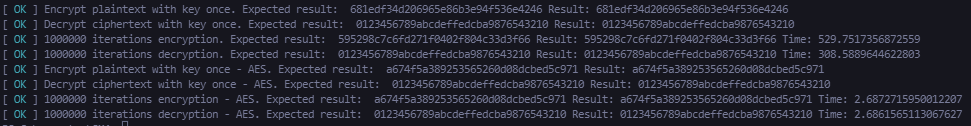
\includegraphics[scale=0.7]{diagramy/testy.PNG}
  \caption{Testy algorytmu szyfrowania SM4}
  \label{fig:SM4}
\end{figure}

\subsection{ Porównanie wydajności }

Planem analizy wydajności, było przeprowadzanie takie samej liczby testów, z tym samym słowem i kluczem, dla algorytmu SM4 oraz AES, ponieważ oba te algorytmy to szyfry blokowe. Aby to zrobić zmierzyliśmy czas wykonywania wszystkich iteracji dla każdego algorytmu i wyliczyliśmy średnia przepływność tych algorytmów. Otrzymane wyniki zaprezentowaliśmy w tabeli  \ref{table:AES_to_SM4}.

\begin{table}[h!]
\centering
\caption{Porównanie przepływności}
\label{table:AES_to_SM4}
\begin{tabular}{ | c | c | c | } 
\hline
 Metoda & Algorytm SM4 [MB/s]& Algorytm AES [MB/s] \\
\hline
$Szyfrowanie$ & 0,03 & 5,68 \\
$Deszyfrowanie$ & 0,05 & 5,68\\
\hline
\end{tabular}
\end{table}

Algorytm AES jest zdecydowanie szybszym algorytmem niż algorytm SM4, ponad 100-krotnie. Fakt, że algorytm SM4 nie został jeszcze złamany, świadczy o jego atrakcyjności ze względu na poziom bezpieczeństwa, jednak pod względem wydajności, w przypadku naszej implementacji, zdecydowanie lepiej prezentuje się algorytm AES. Tak duża różnica w wydajności może być spowodowana implementacją SM4 w języku Python, który jest językiem interpretowanym. Z dużym prawdopodobieństwem lepsze rezultaty uzyskałaby implementacja w języku kompilowanym takim jak np. C.
\newpage
\renewcommand\refname{Bibliografia}

\begin{thebibliography}{99}
\bibitem{SideChannel} Lei, Q., Wu, L., Zhang, S., Zhang, X., Li, X., Pan, L. and Z. Dong:
\emph{Software Hardware Co-design for Side-Channel Analysis Platform on Security Chips},
December 2015
\bibitem{Multi} Biryukov, A., De Canniere, C., Quisquater, M.:
\emph{On Multiple Linear Approximations},
2004
\bibitem{SCA} State Cryptography Administration of China:
\emph{State Cryptography Administration of Chinas},
December 2017
\bibitem{SM4} Translated and typeset by Whitfield Diffie of Sun Microsystems
and George Ledin of Sonoma State University: \emph{SMS4 Encryption Algorithm for Wireless Networks},
15 May 2008

\end{thebibliography}




%------------------------------------------------------------------------
%bibliografia
\newpage
%\bibliographystyle{plabbrv} % plplain plabbrv plalpha
%\bibliography{SYCYF_proj}
\printbibliography[title={Bibliografia}]
	
\end{document}